\chapter{Orchestration-Driven SOA}
\label{bab:odsoa}

\section*{Tujuan Pembelajaran}

\begin{enumerate}
  \item Menjelaskan taksonomi empat lapisan layanan beserta tugas mesin
    orkestrasi yang merangkainya.
  \item Membedakan alur kerja yang tertulis pada satu tempat dari alur kerja
    yang tersebar di dalam layanan, lalu menentukan kapan masing-masing layak
    dipilih.
  \item Mengukur tambahan lompatan akibat mesin orkestrasi, biaya menyisipkan
    satu langkah baru, dan jumlah alur kerja yang terdampak ketika satu layanan
    berubah.
\end{enumerate}

\section{Pendahuluan}

\textit{Orchestration-driven service-oriented architecture} menata sebuah
sistem menjadi beberapa lapisan layanan yang dirangkai satu mesin orkestrasi.
Layanan dibagi menurut seberapa luas pemakaiannya, mulai dari layanan yang
melayani seluruh perusahaan sampai layanan yang hanya melayani satu aplikasi.
Mesin orkestrasilah yang memanggil layanan itu satu per satu menurut urutan
yang sudah dituliskan.

Bentuk ini lahir pada masa integrasi sistem perusahaan, yaitu ketika satu
organisasi memiliki puluhan aplikasi yang saling terpisah. OASIS menyusun model
acuan yang mendefinisikan layanan sebagai mekanisme mengakses satu kemampuan
lewat antarmuka yang sudah disepakati~\cite{oasis2006soarm}. Urutan langkahnya
sendiri ditulis dalam bahasa tersendiri, misalnya Web Services Business Process
Execution Language (WS-BPEL), lalu dijalankan sebuah
mesin~\cite{oasis2007wsbpel}. Hohpe dan Woolf menyebut komponen semacam itu
\textit{process manager}, yaitu satu tempat yang memegang seluruh urutan
pemanggilan sekaligus keadaan setiap proses~\cite{hohpe2003eip}.

Dua hal membuat bentuk ini berbeda dari Bab~11 dan
Bab~13. Yang pertama, pemakaian ulang didorong sejauh
mungkin, sehingga satu layanan sengaja dipakai banyak alur kerja sekaligus.
Yang kedua, seluruh alur kerja tertulis di dalam mesin orkestrasi, bukan
tersebar di dalam layanan. Bab ini mengukur harga kedua pilihan tersebut dengan
angka, mengikuti kerangka yang disusun Richards dan
Ford~\cite{richards2020fundamentals}.

\section{Empat Lapisan Layanan}

Taksonomi layanannya terdiri atas empat tingkat. \textbf{\textit{Business
service}} adalah pintu masuk sebuah proses bisnis, dan isinya hanya urutan
langkah tanpa satu baris aturan bisnis pun. \textbf{\textit{Enterprise
service}} memuat kemampuan yang dipakai banyak proses bisnis sekaligus,
misalnya pemeriksaan nasabah. \textbf{\textit{Application service}} memuat
kemampuan yang hanya dibutuhkan satu aplikasi, misalnya penyusunan bukti
pesanan. \textbf{\textit{Infrastructure service}} memuat kemampuan teknis yang
dipakai semua orang, misalnya pencatatan audit.

Gambar~\ref{fig:taksonomi-odsoa} menunjukkan susunannya. Mesin orkestrasi
berdiri tepat di bawah lapisan pertama, sebab mesin itulah yang membaca urutan
langkah lalu memanggil layanan di bawahnya.

\begin{figure}[htbp]
  \centering
  \begin{tikzpicture}[
    lapis/.style={draw, rounded corners=2pt, minimum width=11cm,
      minimum height=0.85cm, align=center, font=\scriptsize\bfseries},
    kecil/.style={draw, rounded corners=2pt, minimum width=3.55cm,
      minimum height=1.05cm, align=center, font=\scriptsize\bfseries},
    panah/.style={-{Stealth[length=2mm]}, thick}
  ]
    \node[lapis, fill=praditagreen!25] (bisnis) {\textit{business service}\\
      {\tiny\mdseries lima definisi alur kerja, tanpa aturan bisnis}};
    \node[lapis, fill=praditagreen!15, below=0.45cm of bisnis] (mesin)
      {mesin orkestrasi\\
      {\tiny\mdseries membaca urutan, memanggil layanan, mencatat keadaan}};

    \node[kecil, fill=green!10, below=0.55cm of mesin] (app)
      {\textit{application service}\\
      {\tiny\mdseries bukti}\\
      {\tiny\mdseries satu alur kerja saja}};
    \node[kecil, fill=blue!8, left=0.2cm of app] (ent)
      {\textit{enterprise service}\\
      {\tiny\mdseries nasabah, kurs, batas,}\\
      {\tiny\mdseries saldo, transaksi}};
    \node[kecil, fill=green!10, right=0.2cm of app] (inf)
      {\textit{infrastructure service}\\
      {\tiny\mdseries audit}\\
      {\tiny\mdseries seluruh alur kerja}};

    \draw[panah] (bisnis) -- (mesin);
    \draw[panah] (mesin.south) -- ++(0,-0.25) -| (ent.north);
    \draw[panah] (mesin.south) -- ++(0,-0.25) -| (app.north);
    \draw[panah] (mesin.south) -- ++(0,-0.25) -| (inf.north);
  \end{tikzpicture}
  \caption{Taksonomi empat lapisan layanan pada contoh bab ini. Seluruh panah
    berangkat dari mesin orkestrasi, dan tidak ada panah antar layanan}
  \label{fig:taksonomi-odsoa}
\end{figure}

Pembagian tersebut menentukan seberapa banyak alur kerja boleh memakai sebuah
layanan. Tabel~\ref{tab:lapisan-layanan} merangkum ketujuh layanan pada contoh
bab ini beserta jumlah pemakainya, dan angkanya dihitung skrip
\texttt{ukur\_pemakaian.py} dari kelima definisi alur kerja.

\begin{table}[htbp]
  \centering
  \caption{Ketujuh layanan beserta lapisan dan jumlah alur kerja pemakainya}
  \label{tab:lapisan-layanan}
  \begin{tabularx}{\textwidth}{|l|l|l|X|}
    \hline
    \textbf{Layanan} & \textbf{Lapisan} & \textbf{Dipakai} & \textbf{Kemampuannya} \\
    \hline
    \texttt{nasabah} & \textit{enterprise} & 4 dari 5 & Memastikan nasabah terdaftar dan aktif \\
    \hline
    \texttt{kurs} & \textit{enterprise} & 3 dari 5 & Menghitung kurs jual dan nilai rupiah \\
    \hline
    \texttt{batas} & \textit{enterprise} & 2 dari 5 & Menolak pesanan yang melewati pagu harian \\
    \hline
    \texttt{saldo} & \textit{enterprise} & 3 dari 5 & Memotong saldo rupiah nasabah \\
    \hline
    \texttt{transaksi} & \textit{enterprise} & 4 dari 5 & Menulis satu baris ke buku transaksi \\
    \hline
    \texttt{bukti} & \textit{application} & 1 dari 5 & Menyusun teks bukti pemesanan valuta asing \\
    \hline
    \texttt{audit} & \textit{infrastructure} & 5 dari 5 & Menyimpan jejak alur kerja yang selesai \\
    \hline
  \end{tabularx}
\end{table}

Angka pada kolom ketiga sudah memperlihatkan watak setiap lapisan. Layanan
infrastruktur dipakai seluruh alur kerja, layanan perusahaan dipakai sebagian
besar, sedangkan layanan aplikasi hanya dipakai satu. Seksi berikutnya
memperlihatkan siapa yang memanggil ketujuhnya.

\section{Mesin Orkestrasi sebagai Tempat Alur Kerja}

Mesin orkestrasi memegang dua hal yang tidak dipegang layanan mana pun. Yang
pertama adalah urutan langkah setiap alur kerja. Yang kedua adalah keadaan
setiap proses yang sedang berjalan, yaitu langkah mana yang sudah selesai
beserta konteks terakhirnya. Layanan sendiri hanya tahu cara mengerjakan satu
langkah, dan sama sekali tidak tahu langkah apa yang datang sesudahnya.

Listing~\ref{lst:definisi-alur} memperlihatkan kelima definisi alur kerja pada
contoh bab ini. Isinya memang hanya nama langkah beserta urutannya.

\begin{lstlisting}[style=PythonStyle, caption={Definisi kelima alur kerja,
  tersedia di \berkas{sources/chapter12/orkestrator.py}},
  label=lst:definisi-alur]
DEFINISI_ALUR = {
  "pesan-valas": ["nasabah", "kurs", "saldo", "transaksi", "bukti", "audit"],
  "kirim-remitansi": ["nasabah", "kurs", "batas", "saldo", "transaksi",
                      "audit"],
  "bayar-tagihan": ["nasabah", "batas", "saldo", "transaksi", "audit"],
  "tukar-poin": ["nasabah", "transaksi", "audit"],
  "laporan-kurs": ["kurs", "audit"],
}
\end{lstlisting}

Analogi yang mendekati adalah loket satu pintu di bagian akademik. Mahasiswa
menyerahkan berkasnya sekali saja kepada petugas loket. Petugas itulah yang
membawa berkasnya ke bagian keuangan, kembali ke mejanya, lalu membawanya ke
perpustakaan, dan kembali lagi. Langkah kakinya memang lebih banyak daripada
bila berkasnya diserahkan berantai dari satu meja ke meja berikutnya. Akan
tetapi petugas loket selalu mengetahui berkas itu sedang berada di meja mana,
sehingga mahasiswa cukup bertanya kepada satu orang.

Gambar~\ref{fig:kelas-odsoa} menunjukkan hubungan mesin dengan ketujuh
layanannya sebagai diagram kelas. Perhatikan bahwa tidak ada satu pun panah
antar layanan.

\begin{figure}[htbp]
  \centering
  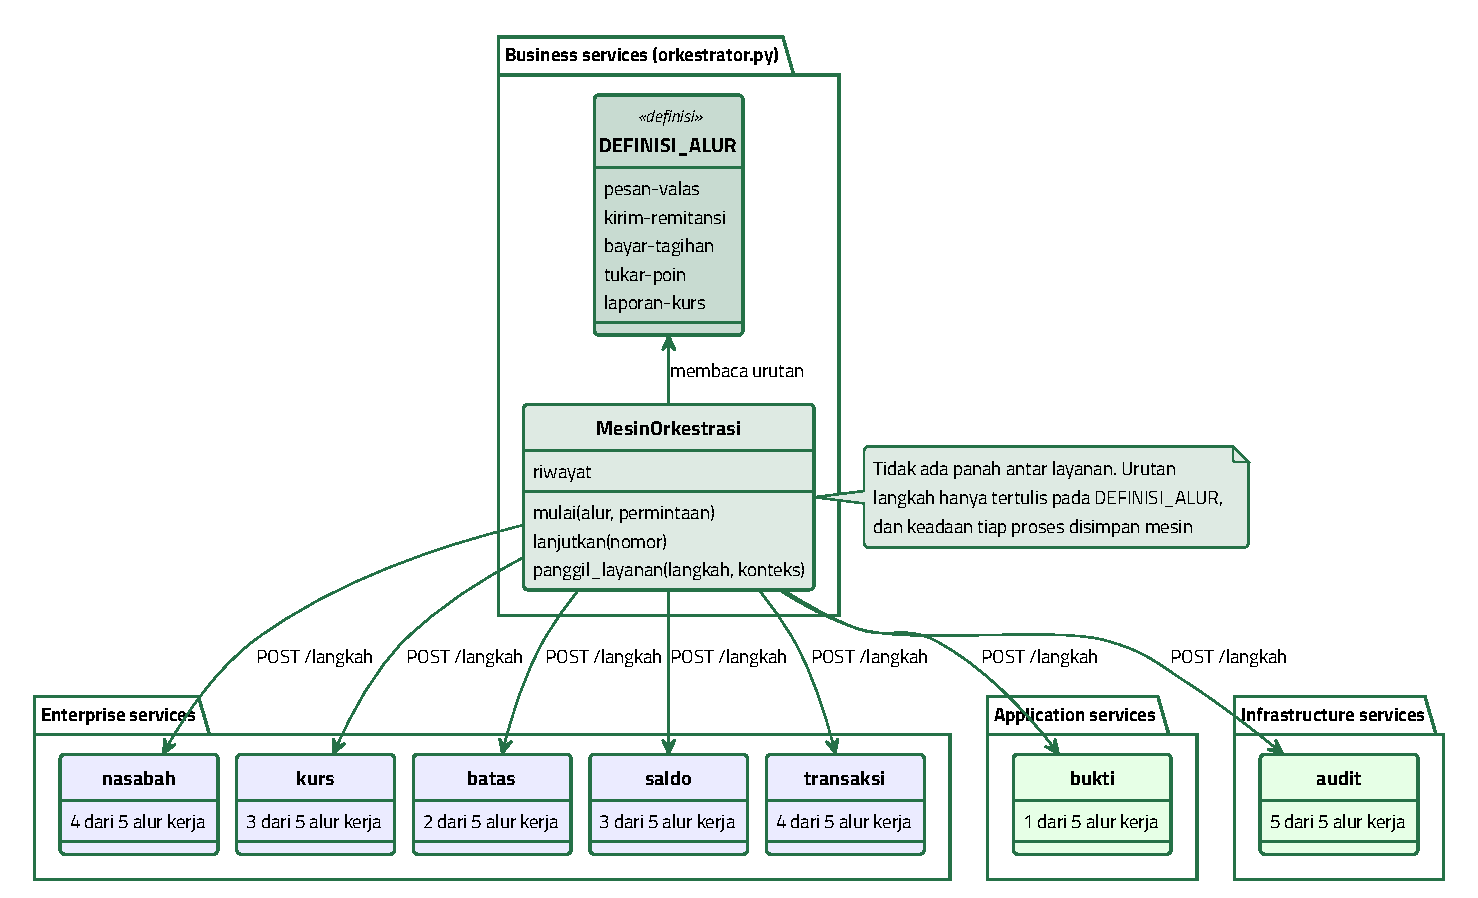
\includegraphics[width=\textwidth, height=0.42\textheight,
    keepaspectratio]{kelas-odsoa.pdf}
  \caption{Mesin orkestrasi memanggil ketujuh layanan, sedangkan urutan
    langkahnya hanya tertulis pada \texttt{DEFINISI\_ALUR}}
  \label{fig:kelas-odsoa}
\end{figure}

Susunan tersebut punya dua konsekuensi praktis. Pertama, mengubah proses bisnis
berarti menyunting satu berkas definisi, bukan menyunting layanan yang sedang
melayani pemakai. Kedua, setiap langkah menempuh dua perjalanan, yaitu dari
mesin menuju layanan lalu kembali lagi ke mesin. Konsekuensi kedua itulah yang
menimbulkan persoalan berikutnya. Pertanyaannya, seberapa mahal perjalanan
pulang itu sebenarnya.

\section{Lompatan yang Dibayar}

Jawabannya dapat dihitung, sebab jumlah lompatan jaringan adalah bilangan
bulat. Versi orkestrasi menempuh satu lompatan menuju mesin ditambah satu
lompatan untuk setiap langkah. Versi tanpa orkestrasi menempuh satu lompatan
menuju layanan pertama, lalu satu lompatan untuk setiap penerusan. Alur kerja
enam langkah karena itu menempuh tujuh lompatan pada versi pertama dan enam
lompatan pada versi kedua.

Gambar~\ref{fig:sekuens-odsoa} membandingkan keduanya. Bagian atas
memperlihatkan konteks yang kembali ke mesin sesudah setiap langkah, sedangkan
bagian bawah memperlihatkan konteks yang diteruskan langsung.

\begin{figure}[htbp]
  \centering
  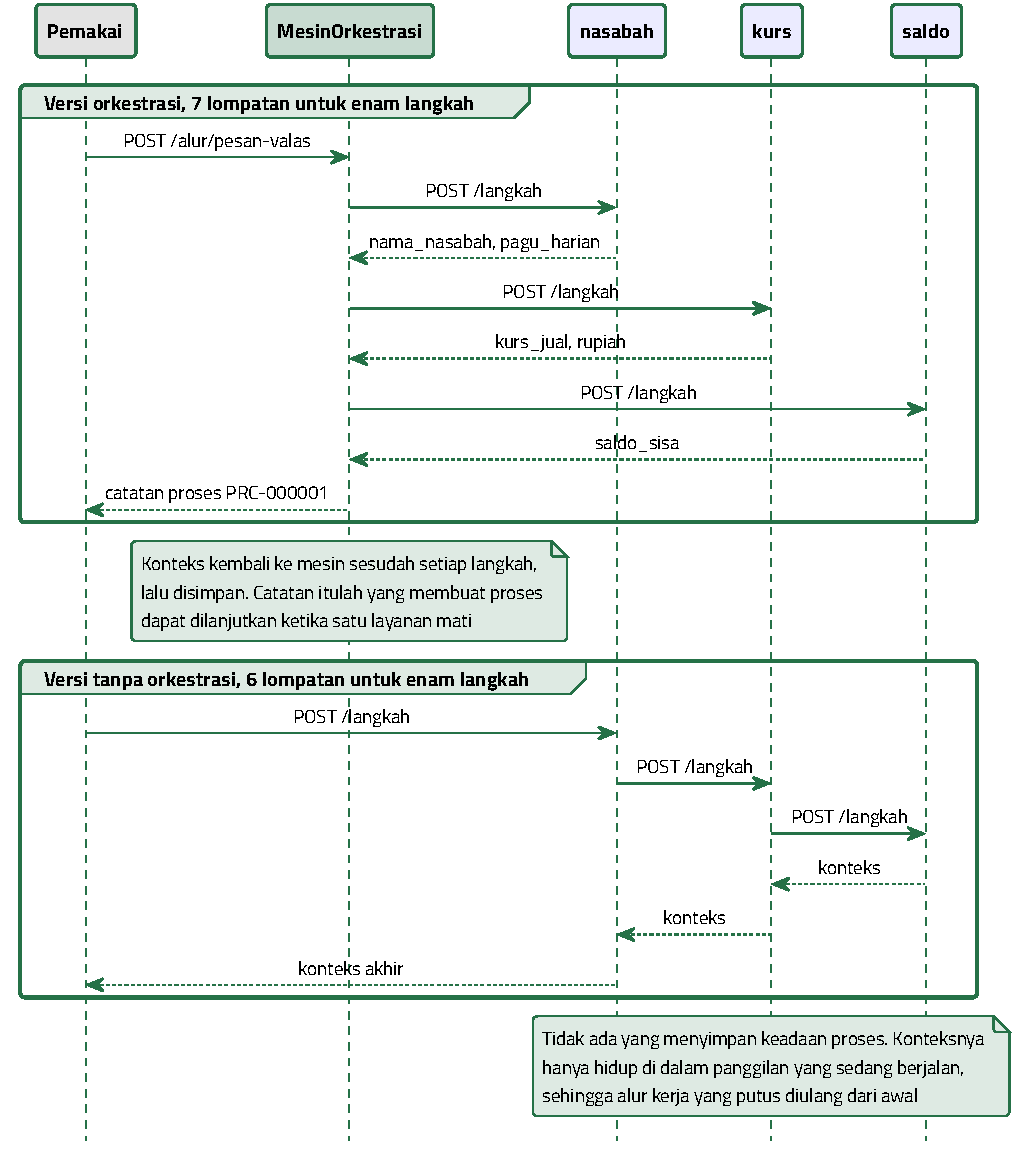
\includegraphics[width=0.86\textwidth, height=0.54\textheight,
    keepaspectratio]{sekuens-odsoa.pdf}
  \caption{Tiga langkah pertama pada kedua versi. Versi orkestrasi selalu
    kembali ke mesin, sedangkan versi tanpa orkestrasi tidak pernah kembali}
  \label{fig:sekuens-odsoa}
\end{figure}

Angkanya tidak diperkirakan, melainkan dicacah. Setiap layanan dan mesin
orkestrasi menambah satu pencacah bersama ketika melayani satu permintaan
Hypertext Transfer Protocol (HTTP), lalu pencacah itu dibaca sesudah satu alur
kerja selesai. Hasilnya tujuh berbanding enam, yaitu tambahan satu lompatan
atau 16,7 persen.

Pertanyaan berikutnya, seberapa besar tambahan satu lompatan itu terasa pada
waktu. Skrip \texttt{ukur\_lompatan.py} menjalankan dua ratus alur kerja pada
masing-masing versi secara bergantian, lalu melaporkan sebaran waktunya.
Tabel~\ref{tab:latensi-odsoa} memuat hasil satu kali pengukuran nyata.

\begin{table}[htbp]
  \centering
  \caption{Latensi dan lompatan kedua versi, dua ratus alur kerja}
  \label{tab:latensi-odsoa}
  \begin{tabularx}{\textwidth}{|X|l|l|}
    \hline
    \textbf{Yang diukur} & \textbf{Orkestrasi} & \textbf{Tanpa orkestrasi} \\
    \hline
    Median & 26,467 ms & 22,658 ms \\
    \hline
    Persentil ke-95 & 41,051 ms & 34,575 ms \\
    \hline
    Terbesar & 85,455 ms & 66,492 ms \\
    \hline
    Lompatan per alur kerja & 7 & 6 \\
    \hline
    Putaran lebih cepat & 14 dari 200 & 186 dari 200 \\
    \hline
  \end{tabularx}
\end{table}

Ragam pengukurannya perlu diperiksa lebih dahulu. \textit{Range} di dalam versi
tanpa orkestrasi tercatat 49,903 milidetik, sedangkan selisih median kedua
versi hanya 3,809 milidetik. \textit{Range}-nya 13,1 kali lebih besar daripada
selisih yang dicari, sehingga satu kali pengukuran memang tidak cukup untuk
menyimpulkan apa pun. Pencacahan per putaran yang menjawabnya, yaitu versi
tanpa orkestrasi lebih cepat pada 186 dari 200 putaran.

Ada satu kecocokan yang menarik pada angka tersebut. Biaya satu lompatan pada
versi tanpa orkestrasi adalah 22,658 dibagi enam, yaitu 3,776 milidetik.
Selisih median kedua versi 3,809 milidetik, yaitu hampir tepat satu lompatan.
Tambahan waktunya karena itu memang berasal dari perjalanan pulang ke mesin,
bukan dari pekerjaan tambahan di dalam mesin. Perbandingan waktunya pun sejalan
dengan perbandingan lompatannya, yaitu 1,17 kali melawan 1,167 kali.

Ujung sebarannya bercerita lebih banyak lagi. Selisih pada median 3,809
milidetik, sedangkan selisih pada persentil ke-95 melebar menjadi 6,476
milidetik dan pada nilai terbesar menjadi 18,963 milidetik. Pelebaran itulah
gejala antrean, sebab versi orkestrasi memang menunggu pada satu titik
tambahan. Median saja tidak memperlihatkannya.

\section{Menyisipkan Satu Langkah ke Tengah Alur Kerja}

Proses bisnis jarang bertahan tanpa perubahan. Aturan baru datang, lalu satu
langkah harus disisipkan ke tengah alur kerja yang sudah berjalan. Contoh bab
ini menyisipkan pemeriksaan batas harian sesudah langkah kurs, sebab angka
rupiah yang diperiksanya baru dihitung di sana.

Kedua versi menghadapi permintaan yang sama, tetapi tidak membayar harga yang
sama. Skrip \texttt{ukur\_perubahan.py} membandingkan keadaan sekarang dengan
salinan keadaan sesudah penyisipan yang tersimpan di
\berkas{sources/chapter12/sesudah/}, lalu menghitung selisihnya dengan
\texttt{difflib}. Tabel~\ref{tab:biaya-perubahan} memuat hasilnya.

\begin{table}[htbp]
  \centering
  \caption{Biaya menyisipkan langkah pemeriksaan batas harian ke tengah alur
    kerja \texttt{pesan-valas}}
  \label{tab:biaya-perubahan}
  \begin{tabularx}{\textwidth}{|X|l|l|}
    \hline
    \textbf{Yang dihitung} & \textbf{Orkestrasi} & \textbf{Tanpa orkestrasi} \\
    \hline
    Berkas disunting & 1 & 3 \\
    \hline
    Berkas baru & 0 & 1 \\
    \hline
    Baris berubah & 2 & 25 \\
    \hline
    Layanan lama ikut disunting & 0 & 1 \\
    \hline
    Tempat urutan langkah ditulis & 1 & 6 \\
    \hline
  \end{tabularx}
\end{table}

Baris pertama perlu dibaca dengan hati-hati. Versi orkestrasi memang cukup
menyunting satu baris, sebab layanan \texttt{batas} sudah berjalan dan sudah
dipakai dua alur kerja lain. Kemurahan itu datang dari pemakaian ulang, bukan
dari mesin orkestrasinya sendiri. Bila layanan tersebut belum ada, versi
orkestrasi juga harus membuatnya.

Baris keempat yang tidak dapat ditawar. Versi tanpa orkestrasi wajib menyunting
layanan \texttt{kurs} yang sedang melayani pemakai, sebab layanan itulah yang
memegang nama penerusnya. Menyisipkan langkah baru karena itu menuntut satu
pemasangan ulang layanan lama, sedangkan versi orkestrasi tidak menuntut satu
pun. Listing~\ref{lst:berikutnya} memperlihatkan baris yang dimaksud.

\begin{lstlisting}[style=PythonStyle, caption={Potongan alur kerja yang dipegang
  layanan kurs, tersedia di \berkas{sources/chapter12/berantai/kurs.py}},
  label=lst:berikutnya]
# Potongan alur kerja yang dipegang layanan ini.
BERIKUTNYA = "saldo"


def buat_aplikasi():
  """Membentuk aplikasi Flask layanan kurs beserta penerusnya.

  Mengembalikan objek Flask yang siap dijalankan pada portnya sendiri.
  """
  return pembantu.buat_layanan("kurs", BERIKUTNYA)
\end{lstlisting}

Baris terakhir pada Tabel~\ref{tab:biaya-perubahan} merangkum sebabnya. Urutan
langkah pada versi orkestrasi tertulis di satu berkas, sedangkan pada versi
tanpa orkestrasi tertulis di enam berkas sekaligus. Tidak ada satu berkas pun
di sana yang memuat alur kerjanya secara utuh.

\section{Pemakaian Ulang yang Berlebihan}

Pemakaian ulang adalah alasan utama taksonomi layanan disusun. Satu layanan
perusahaan ditulis sekali lalu dipanggil banyak proses bisnis, sehingga aturan
yang sama tidak ditulis berulang. Richards dan Ford mencatat bahwa dorongan
itulah yang justru menjadi kelemahan terbesar bentuk ini, sebab layanan yang
dipakai bersama menjadi sulit
diubah~\cite{richards2020fundamentals}. Pertanyaannya, seberapa sulit.

Skrip \texttt{ukur\_pemakaian.py} menjawabnya dengan percobaan. Margin pada
layanan \texttt{kurs} dinaikkan lima puluh rupiah per satuan valuta asing, lalu
kelima alur kerja dijalankan ulang dan hasilnya dibandingkan dengan hasil
sebelumnya. Nilai rupiah pesanan \texttt{pesan-valas} berubah dari 163.250
menjadi 163.750. Tabel~\ref{tab:dampak-kurs} memuat sebarannya.

\begin{table}[htbp]
  \centering
  \caption{Akibat menaikkan margin pada satu \textit{enterprise service}}
  \label{tab:dampak-kurs}
  \begin{tabularx}{\textwidth}{|X|l|}
    \hline
    \textbf{Yang dihitung} & \textbf{Nilai} \\
    \hline
    Alur kerja terdaftar & 5 \\
    \hline
    Alur kerja pemanggil \texttt{kurs} & 3 dari 5 \\
    \hline
    Berubah lewat antarmuka layanan & 3 dari 5 \\
    \hline
    Berubah lewat data bersama & 1 dari 5 \\
    \hline
    Wajib diuji ulang & 4 dari 5 \\
    \hline
    Tidak terdampak & 1 dari 5 \\
    \hline
  \end{tabularx}
\end{table}

Baris keempat memuat kejanggalan yang layak diperiksa. Alur kerja
\texttt{bayar-tagihan} sama sekali tidak memanggil layanan \texttt{kurs},
tetapi hasilnya tetap berubah. Sebabnya adalah layanan \texttt{saldo} dan
layanan \texttt{batas}, yang menyimpan satu data bersama bagi seluruh alur
kerja. Pesanan valuta asing yang nilainya berubah membuat sisa saldo dan
pemakaian harian ikut berbeda, lalu perbedaan itu terbaca oleh alur kerja lain.

Akibatnya langsung terasa pada pengujian. Mengubah satu layanan perusahaan
menuntut empat dari lima alur kerja diuji ulang, padahal hanya tiga yang
memanggilnya. Bandingkan dengan layanan \texttt{bukti}, yang hanya dipakai satu
alur kerja, sehingga perubahan di sana cukup diuji pada satu alur kerja saja.
Pemakaian ulang yang luas memang menghemat penulisan kode, sedangkan harganya
dibayar setiap kali kode itu berubah.

\section{Ketika Satu Layanan Mati di Tengah Jalan}

Alur kerja enam langkah memiliki enam kesempatan untuk gagal. Kegagalan pada
langkah pertama tidak merepotkan, sebab belum ada apa pun yang berubah.
Kegagalan sesudah saldo terpotong adalah persoalan yang berbeda.

Kasus berikut memperlihatkan akibatnya. Sebuah bank menjalankan pemesanan
valuta asing lewat rangkaian layanan yang saling memanggil. Pada suatu sore
layanan pencatat transaksi mati karena diskonya penuh. Dua puluh pesanan yang
sedang berjalan berhenti tepat sesudah saldo nasabah terpotong. Petugas
operasional menyalakan kembali layanan itu, lalu menjalankan ulang kedua puluh
pesanan tersebut dari awal, sebab tidak ada catatan yang menyatakan langkah
mana yang sudah selesai. Saldo kedua puluh nasabah terpotong untuk kedua
kalinya, dan pengembaliannya baru selesai tiga hari kemudian.

Skrip \texttt{uji\_kegagalan.py} mengulang kejadian itu dengan sengaja.
Layanan \texttt{transaksi}, yaitu langkah keempat dari enam, dimatikan lalu dua
puluh alur kerja dijalankan pada masing-masing versi. Layanan itu kemudian
dinyalakan kembali, dan pemulihannya diukur. Tabel~\ref{tab:kegagalan} memuat
hasilnya.

\begin{table}[htbp]
  \centering
  \caption{Pemulihan dua puluh alur kerja sesudah layanan transaksi dimatikan}
  \label{tab:kegagalan}
  \begin{tabularx}{\textwidth}{|X|l|l|}
    \hline
    \textbf{Yang dihitung} & \textbf{Orkestrasi} & \textbf{Tanpa orkestrasi} \\
    \hline
    Proses tertahan & 20 & 20 \\
    \hline
    Proses dapat dilanjutkan & 20 & 0 \\
    \hline
    Langkah selesai sebelum mati & 3 & 3 \\
    \hline
    Langkah diulang saat pemulihan & 0 & 60 \\
    \hline
    Permintaan HTTP saat pemulihan & 80 & 120 \\
    \hline
    Saldo terpotong ulang & 0 & 3.265.000 rupiah \\
    \hline
  \end{tabularx}
\end{table}

Kedua versi kehilangan jumlah proses yang sama, yaitu dua puluh, dan keduanya
sempat menyelesaikan tiga langkah. Yang membedakan adalah apa yang tersisa
sesudah kegagalan. Mesin orkestrasi menyimpan konteks setiap proses sesudah
tiap langkah, sehingga kedua puluh proses dapat dilanjutkan dari langkah
keempat. Versi tanpa orkestrasi tidak menyimpan apa pun, sebab konteksnya hanya
hidup di dalam panggilan HTTP yang sudah selesai.

Baris terakhir adalah akibatnya. Mengulang alur kerja dari awal berarti
memotong saldo untuk kedua kalinya, dan jumlahnya 3.265.000 rupiah untuk dua
puluh pesanan kecil. Angka itu berasal dari pembacaan saldo sebelum dan sesudah
pemulihan, bukan dari perkiraan. Kemampuan melanjutkan proses karena itu bukan
kemewahan, melainkan alasan paling kuat memelihara sebuah mesin orkestrasi.

\section{Ringkasan}

\textit{Orchestration-driven service-oriented architecture} menata layanan
menjadi empat lapisan lalu merangkainya dengan satu mesin. Lapisan paling atas
hanya memuat urutan langkah, sedangkan kemampuan sesungguhnya berada di lapisan
perusahaan, aplikasi, dan infrastruktur. Mesin orkestrasilah yang membaca
urutan itu lalu memanggil layanan satu per satu.

Yang membuat susunan tersebut bekerja adalah letak pengetahuan. Urutan langkah
tertulis di satu berkas, dan layanan sama sekali tidak mengenal tetangganya.
Karena itu menyisipkan satu langkah ke tengah alur kerja cukup menyunting satu
berkas definisi, tanpa menyentuh satu pun layanan yang sedang melayani pemakai.
Versi tanpa orkestrasi menuliskan urutannya di enam berkas sekaligus, sehingga
penyisipan yang sama menuntut penyuntingan layanan lama.

Letak pengetahuan itu juga menentukan nasib alur kerja yang putus. Mesin
menyimpan keadaan setiap proses sesudah tiap langkah, sehingga dua puluh proses
yang tertahan dapat dilanjutkan tanpa mengulang satu langkah pun. Versi tanpa
orkestrasi harus mengulang dari awal, dan pengulangan itu memotong saldo
nasabah untuk kedua kalinya sebesar 3.265.000 rupiah.

Harganya dibayar pada dua tempat. Yang pertama adalah lompatan tambahan, sebab
konteks selalu kembali ke mesin sesudah setiap langkah. Alur kerja enam langkah
menempuh tujuh lompatan, dan selisih mediannya 3,809 milidetik, yaitu hampir
tepat biaya satu lompatan. Yang kedua adalah pemakaian ulang yang berlebihan,
sebab satu layanan perusahaan yang berubah menuntut empat dari lima alur kerja
diuji ulang, bahkan alur kerja yang tidak memanggilnya sama sekali.

Pesan utama bab ini karena itu bukan bahwa orkestrasi terpusat selalu lebih
baik, melainkan bahwa orkestrasi terpusat memindahkan pengetahuan tentang
proses ke satu tempat. Pemindahan itu murah ketika proses bisnisnya sering
berubah dan wajib dapat dilanjutkan, lalu menjadi mahal ketika layanannya
dipakai terlalu banyak alur kerja sekaligus.

\section{Latihan}

Ketiga latihan berikut memakai satu basis kode yang sama di
\berkas{sources/chapter12/}, tetapi menyasar tiga masalah yang berbeda.
Latihan~1 mengukur tambahan latensi dan lompatan akibat mesin orkestrasi.
Latihan~2 menghitung biaya menyisipkan satu langkah ke tengah alur kerja.
Latihan~3 memeriksa akibat mengubah layanan yang dipakai banyak alur kerja.
Hasil setiap mahasiswa dapat berbeda, dan yang dilaporkan adalah pola
perbandingannya, bukan angka mutlaknya.

Penyiapannya dijalankan sekali seperti pada Listing~\ref{lst:venv-ch12}. Bab
ini memakai Flask dan requests, keduanya sudah tercantum pada berkas kebutuhan.

\begin{lstlisting}[language=bash, caption={Menyiapkan bahan sebelum ketiga
  latihan, seluruh skrip tersedia di \berkas{sources/chapter12/}},
  label=lst:venv-ch12]
bash sources/siapkan_venv.sh
source .venv/bin/activate
cd sources/chapter12
python klien.py
# Keluarannya: Lompatan orkestrasi    : 7
# Keluarannya: Lompatan berantai      : 6
\end{lstlisting}

Empat belas server dinyalakan sekaligus oleh setiap skrip, yaitu mesin
orkestrasi, tujuh layanan pasif, dan enam layanan berantai. Portnya berada di
rentang 7120 sampai 7137. Bila salah satu port sudah dipakai program lain,
ubah nomornya pada \berkas{sources/chapter12/konfigurasi.py}.

\subsection*{Latihan 1: Mengukur Tambahan Lompatan dan Latensi}

Latihan ini menghitung harga yang dibayar mesin orkestrasi. Kedua versi
menjalankan alur kerja yang sama dan menghasilkan bukti yang sama persis,
sehingga selisihnya benar-benar selisih cara merangkai. Pengukurannya diulang
dua ratus putaran, sebab satu putaran tidak cukup untuk menyimpulkan apa pun.
Langkah kerjanya sebagai berikut.

\begin{enumerate}
  \item Jalankan \texttt{python klien.py}, lalu bandingkan kedua baris
    buktinya. Catat pula kedua angka lompatannya.
  \item Jalankan \texttt{python ukur\_lompatan.py}. Skrip tersebut mencetak
    baris kemajuan setiap empat puluh putaran, sehingga jalannya terlihat.
  \item Catat kelima belas angka pada laporan akhirnya.
  \item Buka \berkas{sources/chapter12/data.py}, lalu tunjukkan fungsi yang
    menambah pencacah permintaan HTTP.
  \item Ubah \texttt{JUMLAH\_PUTARAN} menjadi 50, jalankan ulang, lalu catat
    perubahan pada baris pencacahan putaran.
\end{enumerate}

Tabel~\ref{tab:lat1odsoa-contoh} berisi hasil satu kali pengukuran nyata.

\begin{table}[htbp]
  \centering
  \caption{Contoh hasil Latihan 1 yang sudah terisi, dua ratus alur kerja}
  \label{tab:lat1odsoa-contoh}
  \begin{tabularx}{\textwidth}{|X|l|}
    \hline
    \textbf{Yang dilaporkan} & \textbf{Nilai} \\
    \hline
    Median orkestrasi & 26,467 ms \\
    \hline
    Median tanpa orkestrasi & 22,658 ms \\
    \hline
    Selisih median & 3,809 ms \\
    \hline
    Persentil ke-95 orkestrasi & 41,051 ms \\
    \hline
    Terbesar orkestrasi & 85,455 ms \\
    \hline
    \textit{Range} dibagi selisih & 13,1 kali \\
    \hline
    Tambahan lompatan & 1 dari 6, yaitu 16,7 persen \\
    \hline
    Putaran tanpa orkestrasi lebih cepat & 186 dari 200 \\
    \hline
  \end{tabularx}
\end{table}

Isikan hasil pengukuran pada Tabel~\ref{tab:lat1odsoa-hasil}.

\begin{table}[htbp]
  \centering
  \caption{Lembar isian Latihan 1}
  \label{tab:lat1odsoa-hasil}
  \begin{tabularx}{\textwidth}{|X|l|l|}
    \hline
    \textbf{Yang dilaporkan} & \textbf{Dua ratus putaran} & \textbf{Lima puluh putaran} \\
    \hline
    Median orkestrasi & \dots & \dots \\
    \hline
    Median tanpa orkestrasi & \dots & \dots \\
    \hline
    \textit{Range} dibagi selisih & \dots & \dots \\
    \hline
    Lompatan per alur kerja & \dots & \dots \\
    \hline
    Putaran tanpa orkestrasi lebih cepat & \dots & \dots \\
    \hline
  \end{tabularx}
\end{table}

Jawab tiga pertanyaan berikut dengan menunjuk angka pada tabel. Pertama,
selisih median hampir sama dengan biaya satu lompatan. Tunjukkan
perhitungannya, lalu jelaskan mengapa kecocokan itu masuk akal. Kedua,
\textit{range} di dalam satu versi jauh lebih besar daripada selisih antar
versi. Jelaskan ukuran mana yang lebih dapat dipercaya di sini, beserta
alasannya. Ketiga, bandingkan selisih pada persentil ke-95 dengan selisih pada
median, lalu jelaskan apa yang ditunjukkan pelebaran tersebut.

\subsection*{Latihan 2: Menyisipkan Satu Langkah ke Tengah}

Latihan ini menghitung biaya mengubah proses bisnis yang sudah berjalan.
Langkah yang disisipkan adalah pemeriksaan batas harian, dan tempatnya sesudah
langkah kurs. Langkah kerjanya sebagai berikut.

\begin{enumerate}
  \item Jalankan \texttt{python ukur\_perubahan.py}, lalu catat kelima angka
    pertama pada laporannya.
  \item Buka \berkas{sources/chapter12/orkestrator.py}, lalu bandingkan
    \texttt{DEFINISI\_ALUR} dengan salinannya di
    \berkas{sources/chapter12/sesudah/orkestrator.py}. Tunjukkan baris yang
    berbeda.
  \item Buka \berkas{sources/chapter12/berantai/kurs.py}, lalu tunjukkan baris
    yang wajib disunting agar langkah baru masuk ke rantainya.
  \item Sisipkan sendiri satu langkah \texttt{audit} kedua ke tengah alur kerja
    \texttt{tukar-poin} pada \texttt{DEFINISI\_ALUR}, jalankan
    \texttt{python ukur\_pemakaian.py}, lalu catat berapa berkas layanan yang
    perlu disunting.
\end{enumerate}

Tabel~\ref{tab:lat2odsoa-contoh} berisi hasil satu kali pengukuran nyata.

\begin{table}[htbp]
  \centering
  \caption{Contoh hasil Latihan 2 yang sudah terisi}
  \label{tab:lat2odsoa-contoh}
  \begin{tabularx}{\textwidth}{|X|l|l|}
    \hline
    \textbf{Yang dihitung} & \textbf{Orkestrasi} & \textbf{Tanpa orkestrasi} \\
    \hline
    Berkas disunting & 1 & 3 \\
    \hline
    Berkas baru & 0 & 1 \\
    \hline
    Baris berubah & 2 & 25 \\
    \hline
    Layanan lama ikut disunting & 0 & 1 \\
    \hline
    Tempat urutan langkah ditulis & 1 & 6 \\
    \hline
  \end{tabularx}
\end{table}

Isikan hasil pengukuran pada Tabel~\ref{tab:lat2odsoa-hasil}.

\begin{table}[htbp]
  \centering
  \caption{Lembar isian Latihan 2}
  \label{tab:lat2odsoa-hasil}
  \begin{tabularx}{\textwidth}{|X|l|l|}
    \hline
    \textbf{Yang dihitung} & \textbf{Orkestrasi} & \textbf{Tanpa orkestrasi} \\
    \hline
    Berkas disunting & \dots & \dots \\
    \hline
    Baris berubah & \dots & \dots \\
    \hline
    Layanan lama ikut disunting & \dots & \dots \\
    \hline
    Tempat urutan langkah ditulis & \dots & \dots \\
    \hline
    Langkah sesudah disisipkan & \dots & \dots \\
    \hline
  \end{tabularx}
\end{table}

Jawab tiga pertanyaan berikut dengan menunjuk angka pada tabel. Pertama,
jelaskan mengapa versi orkestrasi cukup menyunting satu baris, lalu sebutkan
syarat yang membuat kemurahan itu berlaku. Kedua, sebutkan berapa layanan yang
sudah berjalan wajib dipasang ulang pada masing-masing versi, lalu jelaskan
akibatnya bagi pemakai yang sedang memesan. Ketiga, bandingkan jumlah tempat
urutan langkah ditulis pada kedua versi, lalu jelaskan mengapa angka itu lebih
menentukan daripada jumlah baris yang berubah.

\subsection*{Latihan 3: Mengubah Layanan yang Dipakai Banyak Alur Kerja}

Latihan ini menguji sisi gelap pemakaian ulang. Satu \textit{enterprise
service} diubah, lalu jumlah alur kerja yang ikut berubah hasilnya dihitung.
Langkah kerjanya sebagai berikut.

\begin{enumerate}
  \item Jalankan \texttt{python ukur\_pemakaian.py}, lalu catat tabel pemakaian
    ulang beserta keenam angka di bawahnya.
  \item Buka \berkas{sources/chapter12/orkestrator.py}, lalu hitung sendiri
    berapa alur kerja yang menyebut layanan \texttt{kurs}.
  \item Ubah \texttt{LAYANAN\_DIUBAH} pada
    \berkas{sources/chapter12/ukur_pemakaian.py} menjadi \texttt{"bukti"},
    jalankan ulang, lalu catat jumlah alur kerja pemakainya.
  \item Naikkan \texttt{MARGIN\_BARU} menjadi lima ratus rupiah, jalankan
    ulang, lalu catat apakah jumlah alur kerja yang terdampak ikut berubah.
\end{enumerate}

Tabel~\ref{tab:lat3odsoa-contoh} berisi hasil satu kali pengukuran nyata.

\begin{table}[htbp]
  \centering
  \caption{Contoh hasil Latihan 3 yang sudah terisi}
  \label{tab:lat3odsoa-contoh}
  \begin{tabularx}{\textwidth}{|X|l|}
    \hline
    \textbf{Yang dihitung} & \textbf{Nilai} \\
    \hline
    Alur kerja pemanggil \texttt{kurs} & 3 dari 5 \\
    \hline
    Berubah lewat antarmuka layanan & 3 dari 5 \\
    \hline
    Berubah lewat data bersama & 1 dari 5 \\
    \hline
    Wajib diuji ulang & 4 dari 5 \\
    \hline
    Pemakai layanan \texttt{bukti} & 1 dari 5 \\
    \hline
    Pemakai layanan \texttt{audit} & 5 dari 5 \\
    \hline
  \end{tabularx}
\end{table}

Isikan hasil pengukuran pada Tabel~\ref{tab:lat3odsoa-hasil}.

\begin{table}[htbp]
  \centering
  \caption{Lembar isian Latihan 3}
  \label{tab:lat3odsoa-hasil}
  \begin{tabularx}{\textwidth}{|X|l|l|}
    \hline
    \textbf{Yang dihitung} & \textbf{Layanan \texttt{kurs}} & \textbf{Layanan \texttt{bukti}} \\
    \hline
    Alur kerja pemanggilnya & \dots & \dots \\
    \hline
    Berubah lewat antarmuka layanan & \dots & \dots \\
    \hline
    Berubah lewat data bersama & \dots & \dots \\
    \hline
    Wajib diuji ulang & \dots & \dots \\
    \hline
    Lapisan taksonominya & \dots & \dots \\
    \hline
  \end{tabularx}
\end{table}

Jawab tiga pertanyaan berikut. Pertama, satu alur kerja berubah hasilnya
padahal tidak memanggil layanan yang diubah. Sebutkan layanan mana yang
menghantarkan perubahan itu, lalu jelaskan caranya. Kedua, bandingkan jumlah
alur kerja yang wajib diuji ulang ketika \textit{enterprise service} diubah
dengan ketika \textit{application service} diubah, lalu jelaskan mengapa
selisihnya sebesar itu. Ketiga, dengan menggabungkan hasil ketiga latihan,
tentukan pada keadaan apa orkestrasi terpusat sepadan dengan lompatan
tambahannya, lalu sebutkan ketiga angka yang menjadi dasar keputusannya.
